\documentclass[11pt,a4paper]{article}

\usepackage{style2017}

\pagestyle{empty}
\author{Yannick Chistel}
\title{DS2}
\newcounter{num}
\addtocounter{num}{1}
\setcounter{nbDS}{1}

\begin{document}

\begin{headDS}
{DS}{20 octobre 2022}{Programmation orientée objet}{T NSI}
\end{headDS}
	


\section*{\textsc{Exercice \thenum } \hfill 7 points}
Une agence immobilière développe un programme pour gérer les biens immobiliers qu'elle propose à la vente.

Dans ce programme, pour modéliser les données de biens immobiliers, on définit une classe \textsf{Bim} avec les attributs suivants:

\begin{itemize}
\item \textsf{nt} de type \textsf{str} représente la nature du bien (appartement, maison, bureau, commerce,...);
\item \textsf{sf} de type \textsf{float} est la surface du bien;
\item \textsf{pm} de type \textsf{float} est le prix moyen par $m^{2}$ du bien qui dépend de son emplacement.
\end{itemize}

La classe \textsf{Bim} possède une méthode \textsf{estime\_prix} qui renvoie une estimation du prix du bien. Le code (incomplet) de la classe \textsf{Bim} est donné ci-dessous:

\begin{center}
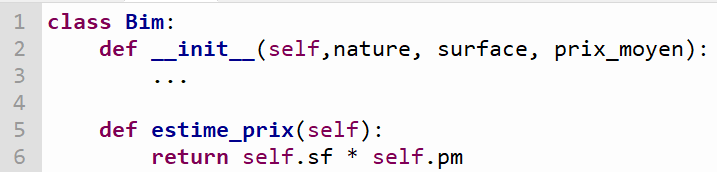
\includegraphics[scale=0.8]{../img/ds_bim_classe.png}
\end{center}

\begin{enumerate}
\item Recopier et compléter le code du constructeur de la classe \textsf{Bim}.

\item On exécute l'instruction suivante: \textsf{b1 = Bim('maison',70.0, 2000.0)}

Que renvoie l'instruction \textsf{b1.estime\_prix()} ? Préciser le type de la valeur renvoyée.

\item On souhaite affiner l'estimation du prix d'un bien en prenant en compte sa nature:

\begin{itemize}
\item pour un bien dont l'attribut \textsf{nt} est \textsf{'maison'} la nouvelle estimation du prix est le produit de sa surface par le prix moyen par $m^{2}$ multiplié par 1,1;
\item pour un bien dont l'attribut \textsf{nt} est \textsf{'bureau'} la nouvelle estimation du prix est le produit de sa surface par le prix moyen par $m^{2}$ multiplié par 0,8;
\item pour les biens d'autres natures, l'estimation du prix ne change pas.
\end{itemize}

Modifier le code de la méthode \textsf{estime\_prix} afin de prendre en compte ce changement de calcul.

\item Écrire le code de la méthode \textsf{nb\_maison(lst)} qui prend en argument une liste Python de biens immobiliers de type \textsf{Bim} et qui renvoie le nombre d'objets de nature \textsf{'maison'} contenus dans la liste \textsf{lst}.

\end{enumerate}
 
%\addtocounter{num}{1}
%\section*{\textsc{Exercice \thenum } \hfill 4 points}



\newpage
\addtocounter{num}{1}
\section*{\textsc{Exercice \thenum } \hfill 6 points}
La classe \textbf{Personnage} permet de créer des personnages identifiés par un nom et munis d'une force. Le nom est une chaine de caractères et la force est un nombre entier. Un personnage peut perdre ou gagner des points de force. Il peut mener un combat avec un autre Personnage pour gagner ou perdre des points de force. \medskip

On donne le code Python de la classe \textbf{Personnage} ci-dessous:
\begin{center}
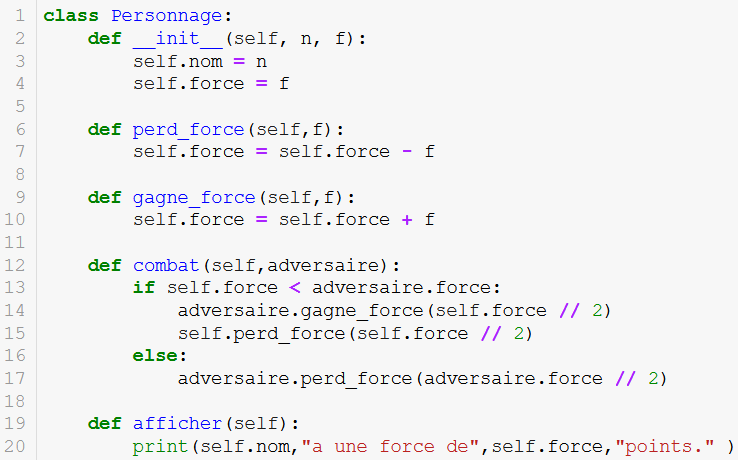
\includegraphics[scale=0.7]{../img/class_personnage.png}
\end{center}
\begin{enumerate}
\item \begin{enumerate}
\item Quels sont les attributs d'un objet créé avec la classe Personnage ?
\item Quelles sont les méthodes de la classe Personnage ?
\end{enumerate}
\item On saisit dans l'interpréteur Python la commande : \textbf{gandalf=Personnage("Gandalf" , 200)}.
\begin{enumerate}
\item Quel est le résultat de cette commande ?
\item Comment peut-on afficher ce personnage ? Quel est alors l'affichage ?
\end{enumerate}
\item On donne le script suivant:
\begin{center}
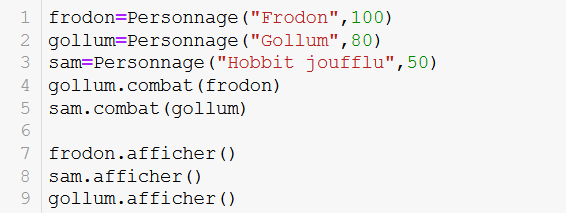
\includegraphics[scale=0.7]{../img/objet_personnage.png}
\end{center}
Quel est l'affichage à l'issu de ce script ?
\end{enumerate}


\newpage
\addtocounter{num}{1}
\section*{\textsc{Exercice \thenum } \hfill 7 points}
On veut créer une classe nommée \textsf{Ville} qui regroupe des informations sur des villes. Pour chacune des villes créées, les informations sont le nom de la ville, le nombre d'habitants et ses coordonnées GPS. Ces informations seront passés en argument dans le constructeur. \medskip

Les attributs de la classe Ville sont les suivants:
\begin{itemize}
\item L'attribut \textsf{nom} est de type \textsf{str};
\item L'attribut \textsf{nbh} est de type \textsf{int};
\item L'attribut \textsf{gps} est un tuple qui contient 2 valeurs de type float associées respectivement à la latitude et la longitude de la ville;
\end{itemize}

Le tableau ci-dessous donne des informations sur trois villes normandes qui seront passées en argument lors de la construction de l'objet Ville.

\begin{center}
\begin{tabular}{|C{3cm}|C{4cm}|C{8cm}|}\hline
\textbf{Nom} & \textbf{Nombre habitants} & \textbf{Coordonnées GPS (latitude, longitude)}\\\hline
Caen & \np{106000} & $(\np{49,18653}~;~\np{-0,36209})$\\\hline
Rouen & \np{110000} & $(\np{49,44879}~;~\np{1,09460})$\\\hline
Le Havre & \np{172000} & $(\np{49,50488}~;~\np{0,12964})$\\\hline
\end{tabular}
\end{center}

On précise que la première coordonnée GPS est la latitude indiquant la position nord-sud et la seconde coordonnée GPS est la longitude indiquant la position est-ouest. \medskip

\begin{enumerate}
\item Écrire en Python le constructeur de la classe \textsf{Ville}.
\item Quelle est l'instruction Python à écrire pour créer la ville \textsf{v1} associée à la ville de Caen du tableau.
\item Écrire la méthode \textbf{afficher} qui renvoie une chaine de caractères affichant le nom de la ville et le nombre d'habitants de la ville. Par exemple, l'instruction \textsf{v1.afficher()} renvoie la chaine \textsf{La ville de Caen a \np{106000} habitants.} \medskip

%\item Quelle commande Python permet d'afficher la ville de Caen?

%\item Soit deux villes dont les coordonnées GPS sont $(lat\_1 ; long\_1 )$ et $(lat\_2 ; long\_2)$. En effectuant les trois calculs suivants, on peut déterminer la distance en kilomètre entre ces deux villes:
%\begin{itemize}
%\item on calcule $x = lat\_2 - lat\_1$
%\item ensuite on calcule $y = (long\_2 - long\_1) \times \cos((lat\_2 - lat\_1) \times \np{0,0087})$
%\item et pour finir $\sqrt{x^{2}+y^{2}}$
%\end{itemize}
\item Une ville est située plus au nord qu'une autre ville si sa latitude est plus élevée. Par exemple, la ville du Havre a une latitude supérieure à la ville de Caen donc Le Havre est plus au nord que Caen. \medskip

La méthode \textbf{plus\_au\_nord\_que} de la classe \textbf{Ville} prend en argument un objet ville et renvoie un booléen. La valeur renvoyée par la méthode est True si la ville à laquelle s'applique la méthode est plus au nord que la ville passée en argument. \medskip

%Par exemple, pour Le Havre qui est plus au nord que Caen, la commande \textbf{le\_havre.plus\_au\_nord\_que(caen)} renvoie \textbf{True} où le\_havre désigne l'objet de la ville du Havre. \medskip
\begin{enumerate}
\item Écrire en Python la méthode \textbf{plus\_au\_nord\_que}.

\item Quelles instructions Python permettent de savoir si la ville de Rouen est plus au nord que Caen ?
\end{enumerate}


%\begin{enumerate}
%\item Que renvoie la commande \textbf{rouen.plus\_au\_nord\_que(le\_havre)} ?
%\item Écrire en Python la méthode \textbf{plus\_au\_nord\_que}.
%\end{enumerate}
\end{enumerate}  



\end{document}
